\chapter{WebRTC}
\label{chap:ch3}

\indent \par Acest capitol are ca scop introducerea în principiile de bază și în componentele proiectului WebRTC, cu menirea de a putea înțelege conceptele următoare. Acoperă API-urile comune, precum și principiile de rețelistică folosite pentru comunicare calitativă, cu latență mică.
\indent \par WebRTC a fost dezvoltat ca standard de către World Wide Web Consortium (W3C) și de către Internet Engineering Task Force (IETF), fiind o colecție open-source de standarde și protocoale. Tehnologiile necesare, precum codecuri și algoritmi de anulare a ecoului, au fost dezvoltate de către o companie suedeză numită Global IP Solutions (GIPS), care a fost mai târziu cumpărată de Google în mai 2010 \cite{WebNSM2017, ACMRTC}. Google a făcut publică implementarea acest proiect în mai 2011 și a propus către IETF standardizarea acestuia. Similar, alți lideri ai industriei precum Mozilla, Ericsson, Microsoft și Apple au furnizat implementări pentru WebRTC, în 2013 fiind realizată interoperabilitatea între browserele Chrome și Firefox \cite{Nyman2013}. Standardul a fost finalizat în ianuarie 2021 și este cunoscut ca RFC 8825.

\section{Arhitectura}
\label{sec:ch3sec1}

% TODO modifică partea asta
\subsection{Stabilirea conexiunilor}
\label{sec:ch3sec1subsec1}
\indent \par La începuturile videoconferințelor pe Internet, protocolul dominant pentru stabilirea conexiunilor între clienți era SIP (Session Initiation Protocol). Însă acesta nu vine inclus cu browserele moderne, așadar este nevoie de a furniza o implementare precum SIP.js \cite{WebNSM2017}. Așadar, WebRTC oferă liberatea dezvoltatorului de a stabili modalitatea prin care doi clienți pot iniția un apel. 
\indent \par Mecanismul prin care se face legătura între aceștia se numește \textit{signaling} (engl. \textit{semnalizare}). Poate fi implementat folosind cereri HTTP, însă prin natura stateless a protocolului HTTP, prin care nu se păstrează informațiile de la cererile anterioare, trebuie trimise continuu cereri, chiar dacă nu se primește sau transmite niciun mesaj nou \cite{WebNSM2017}. Această abordare duce la risipă de lățime de bandă și la o latență ridicată \cite{WebNSM2017}. O soluție ar fi de a inițializa o conexiune WebSocket, care păstrează deschisă legătura cu serverul. Singura responsabilitate a dezvolatorului rămâne de a asigura realizarea schimbului de pachete SDP între clienți și a candidaților ICE, despre care voi discuta în subcapitolul următor. Ca observație, oricare din clienți poate să schimbe sursa conținutului de transmis, organizată pe track-uri separate pentru audio și pentru video - ce vor fi șterse - moment în care se vor renegocia pachetele SDP.

\subsection{Topologii de comunicare}
\label{sec:ch3sec1subsec2}
\indent \par WebRTC este conceput pentru a permite comunicarea directă între participanți, fără a fi nevoie de a transporta pachetele multimedia printr-un server specializat. Totuși, există situații în care această modalitate este dezavantajoasă, acest lucru putându-se specifica la momentul creării conexiunii.
\subsubsection{Mesh}
\label{sec:ch3sec1subsec2subsubsec1}
\begin{figure}[H]
    \centering
    \scalebox{0.65}{\input{figures/webrtc_mesh.pdf_tex}}
    \caption{Topologie mesh într-o sesiune WebRTC}
    \label{WebRTCMesh}
\end{figure}
% TODO finish talks about mesh topology, maybe bring a graph of resource usage in the mesh topology
\indent \par Cea mai simplă topologie este cea mesh (engl. \textit{pânză}) \ref{WebRTCMesh}, în care toți clienții sunt interconectați. Într-o conversație de \(n\) utilizatori, fiecare utilizator va avea \(n-1\) conexiuni deschise, în total fiind \(n*(n-1)\) conexiuni. Această metodă este potrivită doar în pentru \(n\) mic, deoarece fiecare nod va trebui să decodeze \(n-1\) fluxuri de date audio-video, ceea ce crește radical consumul resurselor de către procesor, cu atât mai mult dacă imaginile sunt de calitate înaltă. De asemenea, lățimea de bandă necesară este ridicată, datorită multiplelor fluxuri. În schimb, nu este nevoie de server intermediar, ceea ce reduce costurile de implementare.
\indent \par Se poate particulariza acest scenariu în cazul în care nu toți partajează conținut. Așadar, unele conexiuni nu mai sunt necesare, iar topologia va deveni, după caz, arborescentă. Mai departe, se poate modela în așa fel încât gradul fiecărui nod să fie redus, iar lățimea de bandă folosită să fie scăzută.

\subsubsection{Stea}
\label{sec:ch3sec1subsec2subsubsec2}
\indent \par O altă topologie des întâlnită în implementările aplicațiilor WebRTC este cea de tip stea. În acest caz, fiecare pereche de noduri va fi intermediată de către un server media. Acest server poate manipula conținutul de la fiecare nod, să îl unească într-un singur set de date, sau să îl redistribuie fiecăruia așa cum este. În primul caz, avem de a face cu un multipoint control unit (MCU) \ref{WebRTCStarMCU}, iar în al doilea cu un selective forwarding unit (SFU) \ref{WebRTCStarSFU}.
\begin{figure}[H]
    \centering
    \scalebox{0.65}{\input{figures/webrtc_star_mcu.pdf_tex}}
    \caption{Topologie de tip stea cu server MCU}
    \label{WebRTCStarMCU}
\end{figure}
\indent \par Un avantaj major în cazul topologiei cu server MCU este că fiecare nod trimite și primește câte un singur flux audio-video, ceea ce duce la o economisire de resurse utilizate și de lățime de bandă. Dar există și dezavantaje, și anume, că serverul media va fi consumatorul de resurse, deoarece lui i se atribuie sarcina de a decoda și multiplexa conținutul, ceea ce duce la costuri mai mari de întreținere. Fiind o singură imagine primită, aceasta va fi dificil de prelucrat de către client.
\indent \par Se observă că serverul de signaling poate exista independent de cel media, datorită independenței responsabilităților sale și a posibilității de a specifica mai multe servere media din fiecare nod.
\begin{figure}[H]
    \centering
    \scalebox{0.65}{\input{figures/webrtc_star_sfu.pdf_tex}}
    \caption{Topologie de tip stea cu server SFU}
    \label{WebRTCStarSFU}
\end{figure}
\indent \par Serverul SFU din topologia de mai sus va fi mai puțin costisitor de întreținut față de unul MCU, deoarece consumul de resurse este redus, nemaifiind necesară procesarea datelor. Însă, într-o sesiune cu \(n\) participanți, fiecare va recepționa \(n-1\) fluxuri de date și va trasmite unul, ceea ce crește lățimea de bandă considerabil față de MCU, dar oferă un avantaj clar față de topologia mesh. O îmbunătățire ar putea reprezenta simulcast SFU, prin care fiecare client va transmite imaginea la calități diferite (în condițiile în care toți suportă același codec), dar va cere de la serverul SFU imaginea de calitate potrivită lățimii sale de bandă \cite{SFU2020}. Astfel, clienții care nu dispun de o lățime de bandă largă nu vor compromite calitatea imaginii celor care dispun \cite{SFU2020}. De exemplu, avem patru participanți, doi dintre ei folosind un telefon conectat la date mobile, iar ceilalți conectați de pe laptopuri la rețeaua de acasă. Cei conectați de pe telefoane vor transmite doar imagini de calitate joasă, iar cei de pe laptopuri vor transmite imagini și de calitate înaltă. Cei din urmă își vor vedea imaginile la calitate înaltă, iar ceilalți vor vedea imaginile de la laptopuri la calitate joasă.


\subsubsection{Hibrid}
\indent \par Se pot combina avantajele celor două topologii prezentate anterior, rezultând o distribuție mai eficientă a resurselor utilizate \ref{WebRTCHybrid}. Implicarea unor topologii de tip mesh unite între ele într-o manieră de tip stea are un compromis pe partea latenței, deoarece datele vor avea un drum mai lung de parcurs până la fiecare destinație, însă libertatea de a decide conexiunile directe între participanți este a dezvoltatorului, iar optimizările pe care acesta le poate realiza sunt numeroase. Folosind algoritmi de flux, se poate rezolva problema lățimii de bandă utilizate, iar prin algoritmi de distanță minimă (ex. Bellman-Kalaba), și cea a latenței.
\begin{figure}[H]
    \centering
    \scalebox{0.65}{\input{figures/webrtc_hybrid.pdf_tex}}
    \caption{Topologie de tip hibrid cu server MCU}
    \label{WebRTCHybrid}
\end{figure}

\section{ICE și NAT traversal. Servere STUN și TURN}
\label{sec:ch3sec2}
\indent \par După realizarea schimbului de descriptori SDP, participanții trebuie să stabilească modul de comunicare între ei, deoarece pe traseu poate traversa unul sau mai multe NAT-uri (Network Address Translator), iar adresele lor IP dintr-o rețea nu vor mai fi valide pe altă rețea \cite{rfc8445}. Prin urmare, transportul de date nu ar mai putea fi posibil în mod direct. Pentru aceasta, s-a realizat un protocol numit Interactive Connectivity Estabilishment (ICE). Ideea principală a ICE este că se va folosi un server intermediar (STUN sau TURN), pe care fiecare agent (nod) are o varietate de adrese candidat \cite{rfc8445}.
\indent \par Teoretic, oricare adresă candidat al unui agent poate fi folosită pentru a comunica cu oricare din adresele candidat ale altui agent. În realitate, majoritatea din combinațiile de adrese nu vor funcționa. De exemplu, dacă amândouă nodurile se află în spatele unor NAT-uri, prin adresele interfețelor atașate direct (de pe partea publică a NAT-urilor) nu vor putea comunica direct \cite{rfc8445}. ICE are tocmai acest rol: de a încerca fiecare pereche posibilă de adrese până găsește una sau mai multe care funcționează.
\subsection{Tipuri de candidați}
\indent \par Pentru a face posibil schimbul de conexiuni, un agent trebuie să colecteze una sau mai multe adrese candidat. Adresele candidat sunt perechi de adresă IP și de port pe un protocol de transport specific (de obicei UDP). Există patru tipuri de candidați:
\begin{itemize}
    \item \textit{host} (engl. \textit{gazdă}), care poate comunica direct; este obținut direct de la interfețele locale de rețea (Ethernet, Wi-Fi);
    \item \textit{server-reflexive}, candidat obținut de la un server STUN; este adresa publică a NAT-ului, împreună cu portul pe care NAT-ul îl atribuie când un client trimite cererea de alocare (binding request) către serverul STUN sau TURN \cite{rfc5245};
    \item \textit{peer-reflexive}, candidat obținut de la un server STUN; este adresa publică a NAT-ului, împreună cu portul pe care NAT-ul îl atribuie când clientul primește răspunsul la un binding request de la server, în fazele mai târzii ale ICE;
    \item \textit{relay} (engl. \textit{releu}), candidat obținut de la un server TURN; va conține adresa serverului TURN care va fi responsabil de a retrimite conținutul către cealaltă parte \cite{rfc5245}.
\end{itemize}
\begin{figure}[H]
    \centering
    \scalebox{0.7}{\input{figures/ice_addresses.pdf_tex}}
    \caption{Diagrama adreselor în traseul către serverul TURN}
\end{figure}
\indent \par De observat este că serverele STUN (Session Traversal Utilities for NAT) sunt mai simple decât cele TURN (Traversal Using Relays around NAT), deoarece ele nu au responsabilitatea de a primi pachete de la clienți și de a le redistribui. Cererea ce trebuie trimisă către STUN se numește \textit{binding request} (engl. \textit{cerere de legare}), iar cea către TURN se numește \textit{allocate request} (engl. \textit{cerere de alocare}), cea din urmă având rolul de a aloca un relay pe serverul TURN. 
\indent \par O altă observație este că serverele STUN nu pot fi folosite în cazul unui NAT simetric, deoarece clientului din spatele NAT-ului i se va atribui un port diferit dacă va trimite către o destinație diferită, deși adresa și portul lui sursă rămân neschimbate \cite{rfc5389}.
\indent \par De asemenea, nu se confunda serverele TURN cu cele SFU, deși responsabilitățile lor sunt similare. Clienții trebuie să se conecteze cu serverul SFU ca și cum s-ar conecta cu un alt client, așadar s-ar putea să fie nevoie de un server TURN pe traseul către SFU. Serverul TURN este folosit doar în cazul în care nu se pot conecta la candidații găsiți prin STUN, este un intermediar între clienți sau între clienți și un server media, deci nu poate înlocui un SFU și invers.
\subsection{Obținerea candidaților}
\indent \par Înainte de a proba fiecare conexiune, un agent ICE are nevoie de o listă de candidați. În primă fază, el listează adresele fiecărei interfețe de rețea existente (fizică precum Ethernet, Wi-Fi sau USB, sau virtuale, precum mecanisme de tunelare ca VPN) \cite{rfc8445}. Agentul obține fiecare candidat host prin legarea la un port UDP de pe adresa IP a fiecărei interfețe listate \cite{rfc8445}. 
\indent \par Candidatul host este mereu asociat cu o componentă pentru care este candidat \cite{rfc8445}. Fiecare componentă are asociat un ID. Acest \textit{component ID} va avea valoarea 2 pentru un flux de date (stream) RTCP (RTP Control Protocol) dacă nu este multiplexat pe același port UDP \cite{rfc8445}. În caz contrar, va avea valoarea 1. Pentru RTP (Real-time Transport Protocol) va fi mereu valoarea 1 \cite{rfc8445}. În cazul în care agentul are \(K\) adrese IP și folosește candidați separați pentru RTP și RTCP, va avea \(2*K\) candidați host.
\indent \par Urmează căutarea candidaților server-reflexive și a celor relay. Pentru aceasta, este nevoie de interogarea serverelor STUN și TURN specificate în listă. În unele situații, totuși, nu este nevoie de utilizarea lor \cite{rfc8445}. În acest caz, este recomandat să se implementeze această funcționalitate și să fie doar lăsată dezactivată, deoarece, în timp, se pot schimba cerințele \cite{rfc8445}. 
\indent \par Când sunt specificate mai multe servere STUN sau TURN, agentul ar trebui să returneze candidații pentru cel puțin unul din ele \cite{rfc8445}. Va realiza perechi între fiecare candidat host și fiecare server STUN sau TURN, iar pentru fiecare pereche, va trimite un binding request sau un allocate request \cite{rfc8445}. Agentul va primi un binding sau allocate response \cite{rfc8445}. În cazul unei cereri de alocare, va primi un candidat server-reflexive și un candidat relay \cite{rfc8445}. În cazul în care această cerere eșuează din cauza resurselor insuficiente pe server, va încerca un binding request , care va returna doar candidatul server-reflexive \cite{rfc8445}.
\indent \par Procesul de căutare este controlat de un contor, \(Ta\) \cite{rfc8445}. De fiecare dată când expiră acest contor, agentul poate iniția o nouă cerere către STUN sau TURN. Poate reiniția cererile și în cazul în care acestea returnează o eroare, însă nu la un interval mai scurt de \(Ta\) \cite{rfc8445}. 
\begin{figure}
    \centering
    \scalebox{0.75}{\input{figures/webrtc_sdp_ice_exchange.pdf_tex}}
    \caption{Schimbul de candidați ICE în cadrul unei sesiuni WebRTC}
\end{figure}
\subsection{Calcularea parametrilor pentru candidați}
\indent \par După obținerea candidaților, acesta va calcula un \textit{foundation} pentru fiecare. Acest \textit{foundation} este identic pentru candidații care au aceeași adresă IP (chiar dacă porturile sunt distincte), sunt de același tip, au același protocol de transport (TCP sau UDP), sau dacă adresele IP ale serverelor STUN sau TURN de pe care au fost obținuți sunt identice \cite{rfc8445}.
\indent \par Agentul va calcula și prioritatea fiecărui candidat \cite{rfc8445}. Formula recomandată după care se calculează prioritatea este:
\begin{equation}
    prioritate = 2^24 * preferin\cb{t}\breve{a}Tip + 2^8 * preferin\cb{t}\breve{a}Local\breve{a} + 2^0 * (256 - componentID)
    \label{ICEPriority}
\end{equation}
\par \(preferin\cb{t}\breve{a}Tip\) va fi o valoare între 0 și 126, distinctă pentru fiecare tip de candidat și neapărat mai mare pentru tipul peer-reflexive decât cel server-reflexive. \(preferin\cb{t}\breve{a}Local\breve{a}\) va avea valoarea între 0 și 65535 dacă există adrese IP distincte între candidați sau 65535 dacă există doar una singură. \(componentID\) va fi ID-ul componentei asociate \cite{rfc8445}.
\subsection{Schimbul de informații despre candidați}
\indent \par Agenții ICE trebuie să stabilească modalitatea prin care vor realiza schimbul de informații despre candidați (pentru WebRTC se va folosi, de obicei, WebSocket prin serverul de signaling). De asemenea, trebuie să transmită următoarele informații:
\begin{itemize}
    \item lista de candidați. Pentru fiecare candidat (în această ordine):
    \begin{itemize}
        \item \textit{foundation}-ul ca secvență de cel mult 32 de caractere;
        \item component ID-ul;
        \item protocolul de transport;
        \item coeficientul de prioritate, așa cum este menționat mai sus \ref{ICEPriority};
        \item adresa IP și portul specific protocolului de transport;
        \item tipul candidatului (\textit{host}; \textit{srflx} - server-reflexive; \textit{prflx} - peer-reflexive; \textit{relay});
        \item adresa și portul relative (opționale);
        \item alte atribute (ex.: adresa server-reflexive pentru candidații relay).
    \end{itemize}
    \item Tipul Lite sau Full al candidatului.
    \item Valoarea de stimulare a verificării conexiunii (opțională dacă agentul optează pentru valoarea implicită).
    \item Extensii la nivel de flux media sau sesiune (opțiuni ICE) \cite{rfc8445}.
\end{itemize}
\begin{figure}[H]
    \centering
    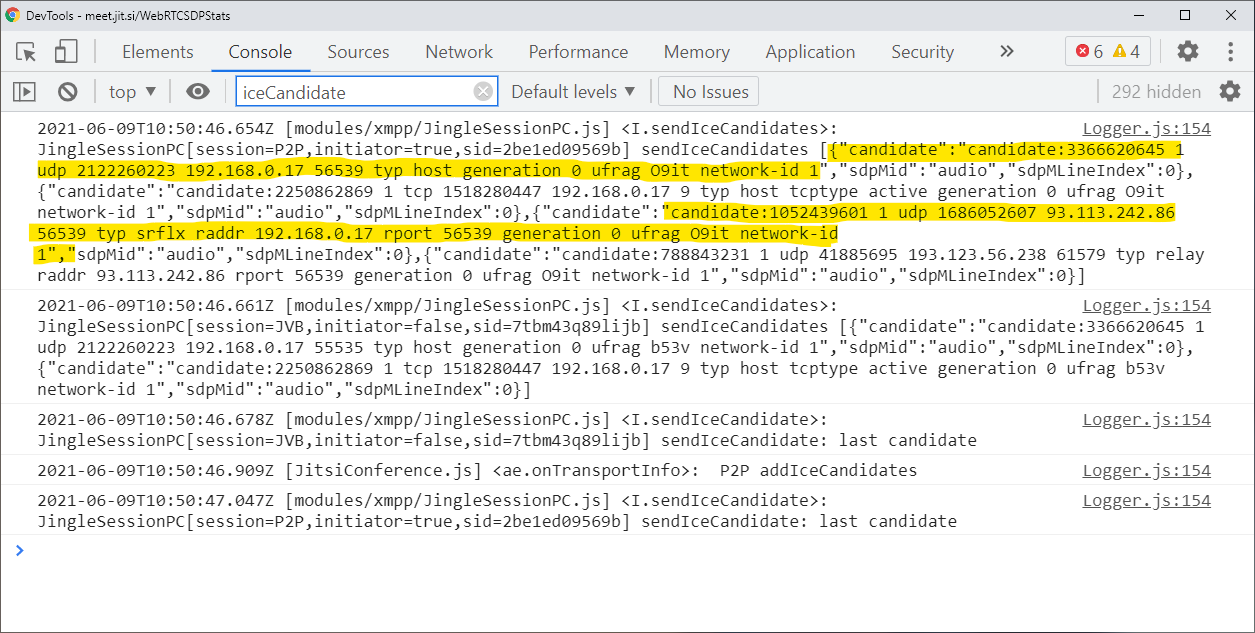
\includegraphics[width=16cm]{figures/ice_exchange_jitsi.png}
    \caption{O listă de candidați ICE dintr-o conversație pe Jitsi Meet}
    \label{ICEExchangeJitsi}
\end{figure}
\indent \par Observând figura de mai sus, se remarcă exact parametrii menționați anterior. Pentru al doilea candidat evidențiat cu galben, foundation-ul său, \texttt{1052439601}, este unic, deoarece candidatul este distinct. Component ID-ul său este \texttt{1}, așadar acesta are cu o componentă de tip RTP atașată. Protocolul de transport ales este \texttt{udp}, iar \texttt{1686052607} reprezintă coeficientul de prioritate . Urmează adresa și IP-ul (\texttt{93.113.242.86}, respectiv \texttt{56539}), atribuite, în acest caz, de către NAT. Următorii parametri sunt cei sunt descriși ca perechi proprietate-valoare. Este menționat \texttt{typ srflx}, deci se specifică faptul că este vorba de tip, respectiv că este server-reflexive. Mai mult, pentru \texttt{raddr 192.168.0.17}, \texttt{raddr} reprezintă mențiunea adresei IP reale a agentului, iar \texttt{192.168.0.17} reprezintă adresa în sine.

\subsection{ICE mismatch}
\indent \par În unele cazuri, poate apărea fenomenul de mismatch (engl. \textit{nepotrivire}), în care un intermediar, cum ar fi un application-level gateway, poate altera informațiile despre candidații ICE \cite{rfc8445}. În această situație, agentul cu care se face schimbul trebuie să poată detecta această alterare și să îl informeze \cite{rfc8445}.

\section{Streaming. Protocoalele SDP și RTP}
\label{sec:ch3sec3}
\indent \par Pentru ca streaming-ul de date să fie posibil, clienții trebuie să stabilească modalitatea prin care ei vor comunica, precum și detalii asupra conținutului pe care îl vor transmite. Pentru acesta, s-a creat protocolul SDP (Session Description Protocol). Este specificat în RFC 4566 și este strict un protocol pentru descriere de sesiuni. Nu incorporează mecanisme de transport, așadar, pentru transmiterea descrierilor, se va folosi alt protocol precum SIP sau WebSocket \cite{rfc4566}. De asemenea, nu suportă negociere de conținut, deoarece se consideră a fi un concept separat de cel al descrierii sesiunilor \cite{rfc4566}.

\subsection{Structura unui descriptor de sesiune SDP}
\indent \par SDP are ca scop oferirea de informații despre streamurile multimedia ce vor permite noilor participanți să se alăture unei sesiuni. \cite{rfc4566}. Streamurile pot fi multicast, așadar vor exista mai mulți clienți care vor transmite unui grup mai larg. În acest caz, SDP deservește și rolul de a comunica existența unei sesiuni \cite{rfc4566}.
\indent \par O descriere SDP conține:
\begin{itemize}
    \item Numele sesiunii și scopul;
    \item Timpul la care sesiunea este activă;
    \item Conținutul multimedia asociat sesiunii;
    \item Informația necesară pentru a primi conținutul (adrese, porturi, formate, codecuri etc.) \cite{rfc4566}.
\end{itemize}
\indent \par De asemenea, este indicată menționarea lățimii de bandă folosită de sesiune și a informațiilor de contact despre persoana responsabilă de sesiune, deoarece resursele participanților pot fi limitate \cite{rfc4566}.
\indent \par Conținutul SDP este descris prin tipul \texttt{application/sdp}, pentru o interpretare corectă de către application-level gateway-uri prin oricare protocol de transport \cite{rfc4566}.
\indent \par Structura sa va fi sub forma unor perechi \texttt{tip=valoare}, delimitate pe rânduri separate și \textbf{fără spațiu} în fața sau în spatele egalului. Fiecare câmp de tip va conține o singură literă mică din alfabetul englez. Fiecare valoare poate conține restul de caractere din setul ISO 10646, cu excepția denumirilor tipurilor de atribute \cite{rfc4566}. Va conține următoarele câmpuri (în această ordine):
\begin{itemize}
    \setlength{\itemsep}{-0.5em}
    \item \texttt{v=  } (versiunea protocolului)
    \item \texttt{o=  } (originea și identificatorul sesiunii)
    \item \texttt{s=  } (numele sesiunii)
    \item \texttt{i=* } (informații despre sesiune)
    \item \texttt{u=* } (URL-ul descrierii)
    \item \texttt{e=* } (adresă e-mail)
    \item \texttt{p=* } (număr de telefon)
    \item \texttt{c=* } (informații despre conexiune; opțional dacă sunt incluse în descriptorii media)
    \item \texttt{b=* } (informații despre lățimea de bandă)
    \item Unul sau mai mulți descriptori temporali
    \item \texttt{z=* } (variațiuni ale fusului orar)
    \item \texttt{k=* } (cheie de criptare)
    \item \texttt{a=* } (una sau mai multe linii; atribute despre sesiune)
    \item Zero sau mai mulți descriptori media
    \setlength{\itemsep}{0em} 
    \item[] \texttt{*} - parametrul este opțional
\end{itemize}
\indent \par Descriptorii temporali vor avea următorul format:
\begin{itemize}
    \setlength{\itemsep}{-0.5em}
    \item \texttt{t=  } (intervalul de timp la care sesiunea este activă)
    \item \texttt{r=* } (numărul de repetări: zero sau mai mult)
\end{itemize}
\indent \par Descriptorii media, în cazul în care există, vor avea următorul format:
\begin{itemize}
    \setlength{\itemsep}{-0.5em}
    \item \texttt{m=  } (numele fluxului media și adresa de transport)
    \item \texttt{i=* } (titlul fluxului)
    \item \texttt{c=* } (informații despre conexiune; opțional dacă este inclus la nivel de sesiune)
    \item \texttt{k=* } (cheia de criptare)
    \item \texttt{a=* } (una sau mai multe linii; atribute despre media)
\end{itemize}
\indent \par Setul de tipuri nu este conceput să fie extensibil, așadar, dacă întâlnește un câmp de tip pe care nu îl recunoaște, va ignora întregul descriptor \cite{rfc4566}. Pentru aceasta, este pus la dispoziție mecanismul \texttt{a=}, al cărui rol este de a extinde SDP și de a-l face potrivit aplicațiilor particulare \cite{rfc4566}.
\begin{lstlisting}[caption={Exemplu de descriptor SDP \cite{rfc4566}}\label{SDPExample}, captionpos=b, label]
    v=0
    o=jdoe 2890844526 2890842807 IN IP4 10.47.16.5
    s=SDP Seminar
    i=A Seminar on the session description protocol
    u=http://www.example.com/seminars/sdp.pdf
    e=j.doe@example.com (Jane Doe)
    c=IN IP4 224.2.17.12/127
    t=2873397496 2873404696
    a=recvonly
    m=audio 49170 RTP/AVP 0
    m=video 51372 RTP/AVP 99
    a=rtpmap:99 h263-1998/90000
\end{lstlisting}
\indent \par Analizând exemplul de mai sus, observăm că, în special pentru câmpurile \texttt{o=}, \texttt{c=} și \texttt{m=}, avem informații ce par criptice la prima vedere. Luând pe bucăți, observăm că \texttt{o=} va conține următorii parametri: numele de utilizator (\texttt{jdoe}), identificatorul sesiunii (\texttt{2890844526}), versiune a sesiunii (\texttt{2890842807}), tipul rețelei (\texttt{IN}, prescurtarea pentru Internet), tipul adresei (\texttt{IP4}, IP versiunea 4), precum și adresa inițiatorului (\texttt{10.47.16.5}).
\indent \par Continuând cu câmpul \texttt{c=}, observăm informații despre conexiune. \texttt{IN} se va regăsi și aici și are acceași semnificație precum la \texttt{o=}, asemenea și tipul \texttt{IP4}. Însă adresa IP arată diferit. Asta se datorează faptului că este o adresă multicast, la care trebuie atașat și TTL-ul (time to live) separat cu o bară oblică.
\indent \par Pentru \texttt{t=}, cele două valori reprezintă numărul de secunde trecute începând cu 1 ianuarie 1900, specific protocolului NTP (Network Time Protocol), reprezentate pe 64 de biți. De observat este că, în anul 2036, se va atinge limita reprezentării în NTP, dar nu va reprezenta o problemă, deoarece SDP folosește reprezentare pe număr arbitrar de cifre.
\indent \par Pentru cele două câmpuri \texttt{m=}, reprezentând descriptorii media, vom avea tipurile de media \texttt{audio} și \texttt{video}. Valorile \texttt{text}, \texttt{application} și \texttt{message} sunt valide. Urmează porturile \texttt{49170}, respectiv \texttt{51372} pe care se va realiza transmisia. Protocolul de transmisie este \texttt{RTP/AVP}, însemnând că RTP folosește profilul audio-video. Se poate întâlni și \texttt{RTP/SAVP}, care se distinge prin faptul că RTP este criptat. Următoarele numere, \texttt{0} și \texttt{99} reprezintă indecși de descriere media și vor avea câte un câmp \texttt{a=} asociat, iar, pentru că se folosește RTP pentru transport, se va regăsi \texttt{rtpmap}. Putem avea mai mulți indecși, prin care putem menționa transmisia a mai multe tipuri de media pe același port. Este menționat codecul \texttt{h263-1998}, împreună cu clock rate-ul (engl. \textit{rata de ceas}) de \texttt{90000}, standard pentru acest codec.

\subsection{RTP}
% TODO termina aici
\indent \par După stabilirea adreselor IP prin care se va realiza transportul conținutului multimedia, trebuie găsită o convenție pentru a-l transporta. Cel mai des folosit protocol de transport este RTP și a fost prima dată specificat în RFC 1889 în ianuarie 1996. Are o strânsă legătură cu RTCP (RTP Control Protocol), destinat transmiterii de feedback asupra calității stream-ului RTP, ceea ce îl face complementar \cite{rfc3550}.
\indent \par RTP nu oferă mecanisme de garantare a transmiterii, lăsând responsabilitatea protocoalelor de nivel mai jos precum UDP, însă folosește numere de secvență pentru ca receptorul să poată reordona corect pachetele sau să determine poziția corectă a pachetului \cite{rfc3550}. Va fi atașat, de obicei, unui port cu număr par între 16384 și 32767 și va forma pereche cu un stream RTCP aflat pe portul imediat următor, cu număr impar.
\indent \par Pachetele RTP respectă următoarea structură:
\begin{figure}[H]
    \centering
    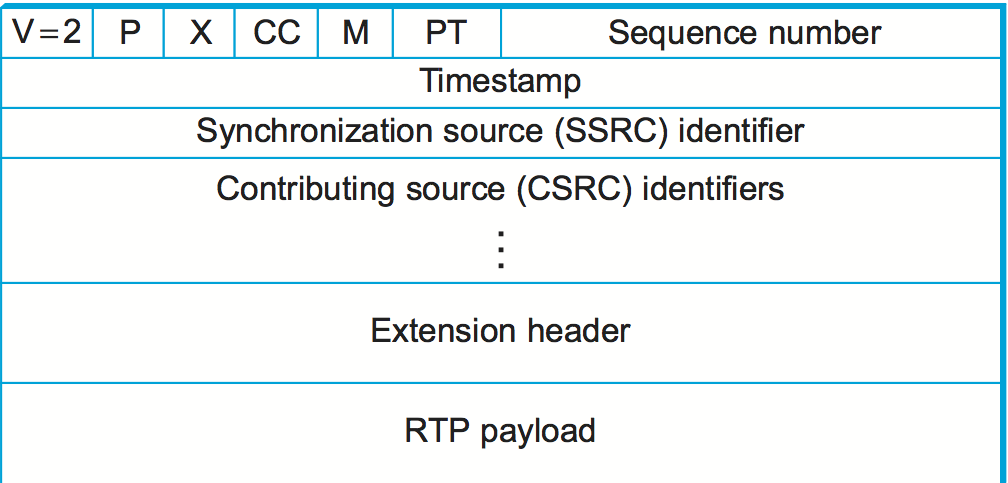
\includegraphics[width=11cm]{figures/rtp_header.png}
\end{figure}
\indent \par De observat este că fiecare rând din tabel va reprezenta câte 4 octeți (32 de biți). De asemenea, există o varietate de parametri ce au următoarea semnificație:
\begin{itemize}
    \item \texttt{V=2} - versiunea 2 a protocolului RTP, va ocupa 2 biți;
    \item \texttt{P} (padding) - bitul de aliniere; va simboliza faptul că pachetul RTP va conține octeți adiționali pentru a-l alinia la o anumită dimensiune, necesară unor algoritmi de criptare; ultimul octet de aliniere va conține numărul de octeți ce trebuie ignorați, inclusiv pe el însuși;
    \item \texttt{X} (extension) - bitul de extensie; va menționa existența unui header (engl. \textit{antet}) de extensie ce se va afla imediat după antetul fix al pachetului RTP;
    \item \texttt{CC} (CSRC Count) - numărul de identificatori CSRC prezenți după antet; va ocupa 4 biți;
    \item \texttt{M} (marker): bit a cărui interpretare variază în funcție de profilul RTP;
    \item \texttt{PT} (payload type) - tipul de conținut transmis în pachetul RTP, va ocupa 7 biți;
    \item sequence number - numărul pachetului RTP; de menționat este că valoarea sa inițială este aleatoare, pentru a îngreuna atacurile criptografice; va ocupa 32 de biți;
    \item timestamp - folosit pentru a marca temporal locul unde ar trebui să fie redat pachetul RTP; asemenea sequence number-ului, valoarea sa inițială trebuie să fie aleatoare;
    \item SSRC (synchronization source) identifier - identificatorul sursei, destinat sincronizării și evitării coliziunilor în cazul în care va primi pachete de la altă sursă;
    \item CSRC (contributing source) identifiers - lista surselor care vor contribui la transmiterea pachetului RTP \cite{rfc3550}.
\end{itemize}

\section{Implementare în browser}
\label{sec:ch3sec4}
\indent \par WebRTC este furnizat cu fiecare browser web popular, precum și cu framework-urile derivate (ex. Electron). Expune mai multe API-uri JavaScript ușor de folosit, care ascund detaliile de implementare și simplifică munca dezvoltatorului. Fiecare API este responsabil de setul său specific de funcții, precum: cameră și microfon, partajarea conținutului ecranului și conexiuni peer-to-peer.

\subsection{Capturarea conținutului media}
\label{sec:ch2sec4subsec1}
\indent \par Pentru a putea realiza streaming-ul audio-video cu un scop, o sursă de conținut este necesară. Media Devices este un numitor comun pentru camerele și microfoanele conectate. În JavaScript, aceste device-uri sunt accesibile prin intermedul interfeței \textit{navigator.mediaDevices}, prin care toate dispozitivele conectate pot fi enumerate, urmărite pentru schimbări, precum și deschise pentru a obține o instanță de MediaStream \cite{WebMedia2014}.
% Please review the last phrase, as it's taken word by word from the official WebRTC page
\indent \par Acest API este folosit prin apelul funcției \textit{mediaDevices.getUserMedia()}, care returnează un promise al cărei funcție de resolve conține un parametru pentru MediaStream-ul asociat dispozitivului. Aceasta cere furnizarea ca parametru un obiect de tip MediaStreamConstraints, prin care constrângeri asupra sursei audio și video se pot specifica, precum și, opțional, identitatea peer, singura care are are acces la stream, unde conținutul este protejat ca și cum regulile CORS cross-origin ar fi în aplicare.
\indent \par O altă opțiune este de a partaja conținutul ecranului. Aceasta este posibilă prin intermediul funcției \textit{mediaDevices.getDisplayMedia()}, foarte similară cu \textit{getUserMedia}, care de asemenea returnează un promise ce rezolvă un MediaStream. Constrângerile sunt diferite: alegerea între multiple opțiuni de a afișa cursorul (mereu, doar când este în mișcare, sau niciodată) și de a afișa zona capturată (întregul ecran, doar o fereastră, sau o filă din browser).
\indent \par Înregistrarea conținutului unui MediaStream este posibilă prin API-ul MediaRecorder, dar în această teză, ne vom concentra doar pe streaming.
\indent \par Vizionarea streamului o chestiune de a crea un elementul HTML \textit{video}, setarea obiectului sursă ca fiind MediaStream-ul și de a furniza o funcție care să redea streamul când metadatele sunt încărcate, ca event handler în proprietatea \textit{onloadedmetadata} din elementul \textit{video}.

\subsection{Inițializarea unei conexiuni peer}
\label{sec:ch3sec4subsec2}

\indent \par Conexiunile peer sunt o parte a specificațiilor WebRTC care ajută la stabilirea unei conexiuni între două aplicații pe două calculatoare diferite pentru a comunica printr-un protocol peer-to-peer. Acestea pot transmite audio, video, sau date bine (cât timp clienții suportă API-ul RTCDataChannel) \cite{WebPeer2014}.
\indent \par Fiecare conexiune peer este gestionată de un obiect RTCPeerConnection, care este instanțiată prin constructorul său specificat ce primește ca parametru un RTCConfiguration, care definește modul în care conexiunea peer este pregătită și care ar trebui să conține informații despre serverele ICE folosite.
\indent \par Pentru inițierea comunicării, este prioritară crearea unei cereri sau unui răspuns SDP, în funcție dacă este vorba despre peer-ul ce apelează, sau despre peer-ul ce răspunde. Apelantul trebuie să trimită obiectul SDP pe care l-a creat peer-ului de la distanță printr-un canal de signaling, diferit de cel prin care se vor transmite datele. Procedura numită signaling nu are o definiție standard.
\indent \par Inițierea unui RTCPeerConnection din apelant cere crearea unui descriptor local, obiect de tip RTCSessionDescription prin metoda \textit{createOffer()} din instanța de RTCPeerConnection. Va fi setat ca fiind descriptor local prin \textit{setLocalDescription()} și va fi trimis la apelat prin canalul de signaling. Apelatul, când primește descriptorul sesiunii, va apela \textit{setRemoteDescription()} și va crea un răspuns la cererea primită cu \textit{createAnswer()} care de asemenea va fi trimis prin canalul de signaling. Inițiatorul apelului va primi răspunsul și îl va seta ca fiind descriptorul remote.

\subsection{Adăugarea stream track-urilor}
\label{sec:ch3sec4subsec3}

\indent \par După crearea unei instanțe de RTCPeerConnection, track-urile de stream trebuie adăugate. Revenind la dispozitivele media și la obiectele sale MediaStream, track-urile sunt conținute într-o listă accesibilă din funcția \textit{getTracks()}. Acestea pot fi adăugate la conexiunea peer cu \textit{addTrack}, care cere instanța streamului \cite{WebStream2014}.
\indent \par Peer-ul care răspunde nu conține o instanță proprie de MediaStream care să conțină track-urile, așadar trebuie să creeze una și să adauge track-urile remote la ea. Un handler de evenimente numit \textit{ontrack} trebuie adăugat. Gestionează câte un track odată. În acest caz, handler-ul va adăuga la instanța nou creată de \textit{MediaStream}, care va fi setată ca obiectul sursă al elementului \textit{video}.
% TODO vorbeste despre renegociere la stergerea de track-uri

\subsection{Obținerea candidaților ICE}
\label{sec:ch3sec4subsec4}

% TODO vorbește despre cum se caută ICE candidates imediat după setLocalDescription și despre trickle ICE
\indent \par Schimbul de informație de conectivitate este obligatoriu înainte ca doi peers pot comunica. Condițiile rețelei pot fi variabile în funcție de un număr de factori (ex. ascunderea adreselor sale IP prin NAT), așadar un intermediar este folosit pentru a descoperi candidații pentru conectarea la peer. Acesta este un serviciu extern și se numește ICE.
\indent \par Imediat după setarea descriptorului local, se va iniția căutarea candidaților ICE, în următoarea ordine: cei host, listând fiecare interfață de rețea (fizică sau virtuală) instalată pe computer, apoi interogând serverele STUN și/sau TURN specificate în câmpul \textit{iceServers} al obiectului de tip RTCConfiguration folosit la crearea obiectului RTCPeerConnection.
\indent \par Fiecare instanță de RTCPeerConnection conține un handler de evenimente pentru noii candidați, numit \textit{onicecandidate}. Va fi apelat de fiecare dată când găsește un candidat nou. Este responsabilitatea dezvoltatorului să îl preia fiecare prin event handler și să îl trimită celuilalt participant la apel, urmând ca acela să îl adauge folosind metoda \textit{addIceCandidate()}.
